\documentclass{article}
\usepackage[utf8]{inputenc}
\usepackage[spanish]{babel}
\usepackage{hyperref}
\usepackage{titlesec}
\usepackage{graphics}
\usepackage{apacite}
\usepackage{amsmath}
\usepackage{amsfonts}
\usepackage{amssymb}
\usepackage{graphicx}
\usepackage{xcolor}
\usepackage{titlesec}
\definecolor{color_uni}{HTML}{800404}
\bibliographystyle{apacite}
\usepackage{parskip}
\usepackage{setspace}
\usepackage{hyperref}
\usepackage[left=2.54cm, right=2.54cm, top=2.54cm, bottom=2.54cm]{geometry}


\title{Materiales modernos}
\author{Francis Joao Huaman}
\date{December 2023}


\begin{document}

%--------------Inicio de monografía--------------%
\begin{titlepage}
    \begin{center}
        {\LARGE \textbf{UNIVERSIDAD NACIONAL DE INGENIER\'IA}}\\
        \vspace{4mm}
        {\Large \text{FACULTAD DE INGENIER\'IA INDUSTRIAL Y DE SISTEMAS}}\\
        \vspace{4mm}
        {\large \text{ESCUELA PROFESIONAL DE INGENIER\'IA DE SISTEMAS}}\\
        \vspace{1mm}
        \begin{figure}[h]
            \centering
            
\includegraphics[height=8.5cm]{assets/img/Logo UNI.png}     
        \end{figure}
        \textcolor{color_uni}{\rule{\linewidth}{0.75mm}}\\
        \begin{spacing}{1}
            \vspace{0.34cm}
            {\LARGE \text{``Materiales modernos II''}}\\
        \end{spacing}
        \textcolor{color_uni}{\rule{\linewidth}{0.75mm}}\\
        \vspace{0.4cm}

    \end{center}

\begin{center}
    {\large \textbf{CURSO:} \text{Qu\'imica I} \hspace{0.5cm} \textbf{SECCIÓN:} \text{A}}\\
    \vspace{0.8cm}
    {\large \textbf{DOCENTES:}}\\
    \vspace{0.4cm}
    {\large \text{CALDERON ZAVALETA, Sandy Luz}}\\
    \vspace{0.4cm}
    {\large \text{REYES ACOSTA, Rosario}}\\
    \vspace{0.8cm}
    {\large \textbf{ALUMNOS:} \hspace{5cm} \textbf{C\'ODIGO:}}\\
    \vspace{0.4cm}
    {\large \text{CRUZ HUAMAN, Francis Joao \hspace{2cm} \text{20237504K}}}\\
    \vspace{2cm}
    {\large \text{LIMA - PER\'U}}\\
    \vspace{0.4cm}
    {\large \text{2023}}\\
\end{center}    

\end{titlepage}
\doublespacing
\tableofcontents


%-------------Contenido de monografía---------------%
\include{secciones/introducción}
\section{Materiales Inteligentes}
\subsection{Aspectos historicos}
Los materiales inteligentes, también conocidos como materiales activos, adaptativos o responsivos, han sido objeto de investigación y desarrollo en diversas disciplinas a lo largo de la historia. Según \cite{materiales} estos materiales tienen la capacidad de responder de manera adaptativa a estímulos externos, como cambios de temperatura, presión, luz, electricidad, entre otros. Aquí hay un breve resumen de algunos hitos históricos en el desarrollo de materiales inteligentes:
    \begin{itemize}
        \item En la década de 1960, se desarrollaron y aplicaron ampliamente materiales piezoeléctricos, que tienen la capacidad de generar una carga eléctrica en respuesta a la aplicación de presión mecánica. Estos materiales se utilizan en sensores y actuadores.
        \item Se produjo un avance significativo con el descubrimiento de polímeros electroactivos, como los polímeros conductores y los electrocerámicos. Estos materiales tienen propiedades eléctricas que pueden ser controladas por estímulos externos.
        \item Los materiales con memoria de forma, como las aleaciones de níquel-titanio (conocidas como Nitinol), fueron desarrollados en esta década. Estos materiales tienen la capacidad de recordar y recuperar su forma original después de ser deformados, lo que ha llevado a aplicaciones en la industria biomédica y aeroespacial.
        \item En las últimas décadas, ha habido un aumento en la investigación de biomateriales inteligentes que responden a estímulos biológicos. Estos materiales se utilizan en aplicaciones médicas, como sistemas de liberación controlada de medicamentos.
        \item Se han desarrollado materiales inteligentes que responden a condiciones ambientales, como cambios de temperatura, humedad o luz solar. Estos materiales tienen aplicaciones en la construcción, la arquitectura y la ingeniería civil.
        \item Los materiales inteligentes tienen aplicaciones en una variedad de campos, incluyendo la robótica, la electrónica flexible, la fabricación avanzada, la industria automotriz y la ingeniería estructural.
    \end{itemize}
\subsection{Métodos de obtención}
    \subsubsection{Síntesis Química}
    Muchos materiales inteligentes se obtienen a través de métodos químicos, que pueden incluir la mezcla y reacción de componentes específicos para formar el material deseado. Esto puede incluir la síntesis de polímeros conductores, compuestos termocrómicos, y otros materiales sensibles a estímulos.
    \subsubsection{Procesamiento de Aleaciones}
    Para materiales con memoria de forma como Nitinol (aleación de níquel-titanio), se utilizan procesos metalúrgicos para obtener la aleación deseada. Esto puede incluir la fusión y solidificación controlada de los metales para lograr las propiedades deseadas.
    \subsubsection{Deposición de Películas Delgadas}
    Para aplicaciones en dispositivos electrónicos y ópticos, se utilizan métodos de deposición de películas delgadas, como la deposición física de vapor (PVD) o la deposición química de vapor (CVD), para producir capas delgadas de materiales con propiedades específicas.
    \subsubsection{Fabricación Aditiva (Impresión 3D)}
    La fabricación aditiva, o impresión 3D, se utiliza para crear estructuras complejas de materiales inteligentes. Puede ser especialmente útil para polímeros y ciertos compuestos sensibles a estímulos.
    \subsubsection{Electroquímica}
    Algunos materiales inteligentes, como electrorreológicos y cromóforos electrocrómicos, se obtienen mediante métodos electroquímicos. Esto implica la manipulación de las propiedades del material mediante la aplicación de corriente eléctrica.
    \subsubsection{Síntesis Biológica}
    En algunos casos, se utilizan métodos biológicos para obtener materiales inteligentes. Esto puede incluir la ingeniería genética de microorganismos o el uso de organismos vivos para producir materiales específicos.
\subsection{Transformaciones de estado}
Los materiales inteligentes exhiben diversas transformaciones de estado en respuesta a estímulos específicos. Estas transformaciones son esenciales para su funcionalidad adaptativa.
    \begin{itemize}
        \item Algunos materiales, como las aleaciones de níquel-titanio (Nitinol) y ciertos polímeros, pueden experimentar un cambio reversible en su forma en respuesta a cambios de temperatura. Este fenómeno se conoce como memoria de forma, y permite a estos materiales recuperar su forma original después de ser deformados.
        \item Los materiales inteligentes a menudo exhiben cambios en sus propiedades eléctricas en respuesta a estímulos externos \cite{castagnino-mat-nanotecnologia}. Los polímeros conductores y los materiales piezoeléctricos son ejemplos. Estos materiales pueden cambiar su conductividad eléctrica o generar una carga eléctrica en respuesta a factores como presión, temperatura o campos eléctricos.
        \item Algunos materiales inteligentes, como los fotocrómicos y termocrómicos, pueden cambiar de color en respuesta a la exposición a la luz o al calor. Estos materiales encuentran aplicaciones en la fabricación de lentes de sol, ropa que cambia de color con la temperatura, entre otras.
        \item Los materiales que responden a la humedad, conocidos como hidrorespóndicos, pueden experimentar cambios en su volumen en presencia de agua. Estos materiales son utilizados en aplicaciones como sensores de humedad y actuadores biomiméticos.
        \item Algunos geles y polímeros inteligentes pueden experimentar un cambio en su rigidez o viscosidad en respuesta a estímulos como cambios de pH, temperatura o concentración iónica. Estos materiales son utilizados en la fabricación de actuadores y dispositivos biomédicos.
        \item Los materiales termoeléctricos pueden cambiar su tamaño en respuesta a cambios de temperatura. Este fenómeno se utiliza en algunos sistemas de refrigeración termoeléctrica y en dispositivos microelectromecánicos (MEMS).
        \item Algunos materiales termocrómicos pueden experimentar un cambio de fase en respuesta a cambios de temperatura, lo que resulta en un cambio en sus propiedades ópticas, como el color. Estos materiales son utilizados en aplicaciones como recubrimientos que indican la temperatura.
    \end{itemize}
\subsection{Clasificación de los Materiales Inteligentes}
    \subsubsection{Materiales con memeria de forma}
    Estos materiales pueden cambiar su forma de manera reversible en respuesta a un estímulo específico, como cambios de temperatura. Este cambio de forma es posible debido a una transformación cristalina reversible en el material.
    \subsubsection{Polimeros inteligentes}
    Los polímeros inteligentes pueden cambiar sus propiedades físicas, químicas o eléctricas en respuesta a estímulos externos. Por ejemplo, algunos polímeros conductores pueden alterar su conductividad eléctrica cuando se exponen a campos eléctricos o cambios de temperatura.
    \subsubsection{Materiales piezoelectricos}
    Los materiales piezoeléctricos generan una carga eléctrica cuando se deforman mecánicamente y, a su vez, experimentan una deformación mecánica cuando se les aplica un campo eléctrico.
    \subsubsection{Materiales Termocrómicos y Fotocrómicos}
    Los materiales termocrómicos cambian de color en respuesta a cambios de temperatura, mientras que los fotocrómicos cambian de color cuando se exponen a la luz. Estos materiales encuentran aplicaciones en gafas, textiles y sensores.
    \subsubsection{Materiales Magnetoestrictivos}
    Los materiales magnetoestrictivos experimentan un cambio en sus dimensiones en respuesta a un campo magnético. Este fenómeno se utiliza en actuadores y sensores magnéticos.
    \subsubsection{Materiales Ópticos cambiantes}
    Cambian sus propiedades ópticas, como la transmitancia de luz, en respuesta a cambios de temperatura o campos eléctricos. Se utilizan en pantallas de cristal líquido y dispositivos ópticos.
    \subsubsection{Materiales Hidrorespóndicos}
    Estos materiales pueden cambiar su volumen en respuesta a cambios en la humedad o la presión de agua. Se utilizan en sensores de humedad y aplicaciones biomédicas.
\subsection{Aleaciones de memoria de forma(SMA)}
Las aleaciones con memoria de forma (SMA, por sus siglas en inglés Shape Memory Alloys) son materiales metálicos que tienen la capacidad única de "recordar" y recuperar su forma original después de haber sido deformados. Este comportamiento se debe a una transición de fase martensítica que ocurre reversiblemente en el material. Entre las aleaciones de memoria de forma más comunes se encuentra la aleación de níquel-titanio, conocida comúnmente como Nitinol.
    \subsubsection{Aplicaciones}
        \begin{itemize}
            \item Stents: Utilizados en cirugía cardiovascular, los stents hechos de SMA se pueden comprimir para la inserción y luego recuperar su forma original una vez colocados en una arteria.
            \item Actuadores en Robótica: Las aleaciones de memoria de forma se utilizan en actuadores para lograr movimientos precisos y controlados en aplicaciones robóticas.
            \item Conectores y Enganches: Se utilizan en aplicaciones industriales y aeroespaciales donde se requieren componentes que se puedan acoplar y desacoplar de manera eficiente.
        \end{itemize}
        
        \begin{figure*}[h]
            \centering
            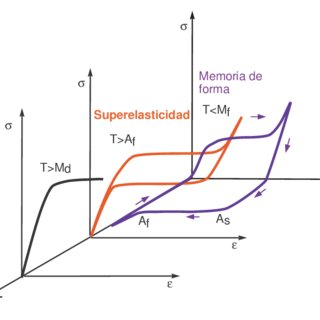
\includegraphics[height=7.8cm]{assets/figures/SMA.jpg}         
        \end{figure*}
\section{Nanotecnologia}
La nanotecnología es un campo multidisciplinario que se centra en la manipulación y control de la materia a una escala extremadamente pequeña, específicamente en el rango de nanómetros, donde un nanómetro es igual a una mil millonésima parte de un metro \cite{nanotecnologia}. Este campo de estudio y aplicación busca comprender, diseñar y utilizar estructuras y dispositivos que operan a nivel nanométrico.

En esencia, la nanotecnología se enfoca en la capacidad de manipular la materia a nivel atómico y molecular para crear nuevos materiales con propiedades únicas y desarrollar dispositivos con funciones específicas. Esto incluye la fabricación y manipulación de nanopartículas, nanotubos, nanocompuestos y otras estructuras a escala nanométrica. La nanotecnología tiene aplicaciones en diversas áreas, como la medicina, la electrónica, la energía, la industria alimentaria, la construcción y muchas más, con el objetivo de mejorar el rendimiento y las características de los materiales y dispositivos a través de la innovación a nivel nanométrico.

    \begin{figure*}[h]
        \centering
        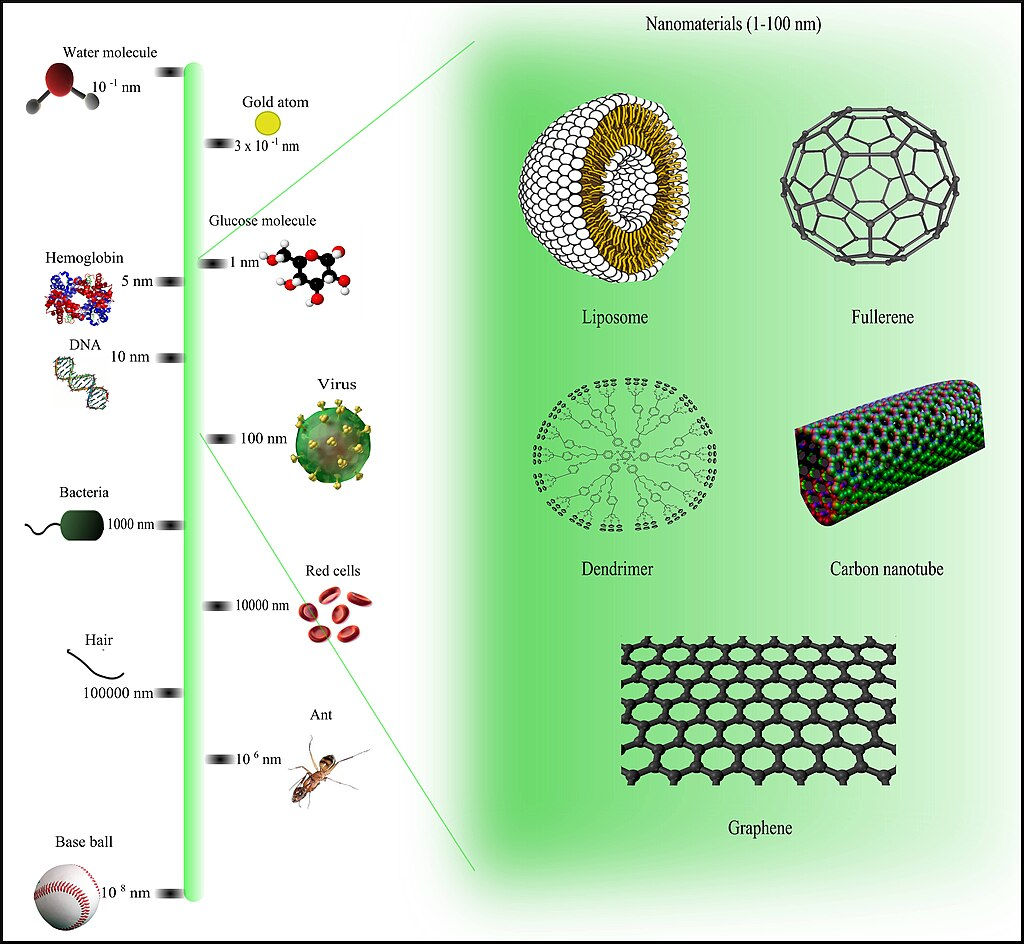
\includegraphics[height=7.8cm]{assets/figures/NAN.jpg}          
    \end{figure*}

\subsection{Materiales nanotecnologicos}
    \subsubsection{Nanopartículas}
    Partículas en el rango nanométrico, que pueden ser de diversos materiales como metales, cerámicas o polímeros. Una de sus caracteristicas es tener una gran relación área-superficie, lo que las hace ideales para aplicaciones como catalizadores, agentes de liberación controlada en medicina y filtros avanzados.
    \subsubsection{Nanotubos de Carbono}
    Estructuras cilíndricas compuestas completamente de carbono, con propiedades eléctricas y mecánicas excepcionales.Se utilizan en la fabricación de materiales compuestos avanzados, como el papel de nanotubos de carbono, y en aplicaciones electrónicas y biomédicas.
    \subsubsection{Grafeno}
    Una capa bidimensional de átomos de carbono dispuestos en una estructura hexagonal.Poseen alta conductividad eléctrica y térmica, y se utiliza en dispositivos electrónicos, baterías, sensores y materiales compuestos.
    \subsubsection{Nanocompuestos}
    Materiales que contienen nanopartículas o nanotubos dispersos en una matriz de otro material.Se caracterizan porque refuerzan las propiedades mecánicas, térmicas y eléctricas del material base, siendo empleados en la fabricación de polímeros reforzados y materiales compuestos avanzados.
    \subsubsection{Dendrímeros}
    Moléculas ramificadas con una estructura dendrítica, utilizadas en nanotecnología para la entrega controlada de fármacos y en la creación de nanoestructuras.
    \subsubsection{Nanocápsulas}
    Estructuras huecas a escala nanométrica utilizadas para encapsular y liberar moléculas específicas. Se aplican en la liberación controlada de medicamentos y en la protección de compuestos sensibles.
\subsection{Aplicaciones}
Los materiales nanotecnológicos tienen una amplia gama de aplicaciones en diversas industrias debido a sus propiedades únicas y a la capacidad de manipular la materia a escala nanométrica. Según \cite{castagnino-mat-nanotecnologia} algunas de las aplicaciones más destacadas de estos materiales:
    \begin{itemize}
        \item Imagen Médica: Agentes de contraste basados en nanomateriales para mejorar la calidad de imágenes médicas, como la resonancia magnética y la tomografía por emisión de positrones
        \item Nanotubos de Carbono y Grafeno: Aplicaciones en dispositivos electrónicos avanzados, como transistores y pantallas flexibles.
        \item Baterías y Almacenamiento de Energía: Uso de nanomateriales para mejorar la capacidad y velocidad de carga de baterías.
        \item Nanopartículas en Envases: Desarrollo de envases nanotecnológicos para prolongar la vida útil de los alimentos y monitorear su frescura.
        \item Nanosensores: Detección precisa de gases, compuestos químicos y biomarcadores para aplicaciones en salud y seguridad.
    \end{itemize}

    \begin{figure*}[h]
        \centering
        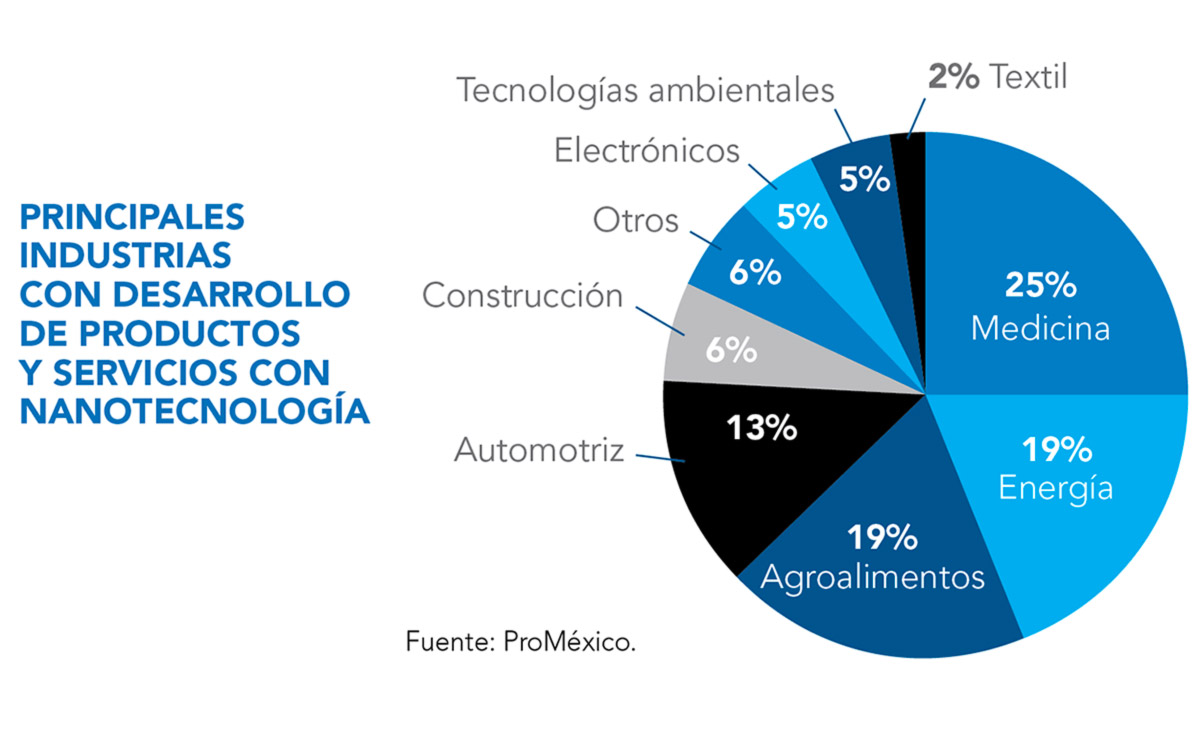
\includegraphics[height=7.8cm]{assets/figures/NANO.jpg}         
    \end{figure*}

\section{Plasma}
El plasma es uno de los cuatro estados fundamentales de la materia, junto con sólido, líquido y gas. A diferencia de estos estados, el plasma se caracteriza por la presencia de partículas cargadas eléctricamente, como iones y electrones, que se comportan de manera colectiva \cite{plasma1}.
\subsection{Propiedades del plasma}
    \subsubsection{Carga electrica}
    La carga eléctrica en el plasma es un fenómeno fundamental que surge de la ionización de los átomos y moléculas presentes en el gas. Cuando se aplica suficiente energía al gas, algunos electrones son arrancados de sus órbitas alrededor de los núcleos atómicos, generando iones positivos (átomos con pérdida de electrones) y electrones libres. Esta separación de cargas crea un ambiente altamente conductor eléctricamente, similar a un gas de electrones y iones. La existencia de estas cargas libres permite que el plasma responda a campos eléctricos y magnéticos, y es la base de muchas de sus aplicaciones prácticas.
    \subsubsection{Temperatura}
    La temperatura elevada en el plasma es una consecuencia directa de la alta energía cinética de las partículas cargadas presentes. En términos simples, la temperatura es una medida de la energía promedio de movimiento de las partículas en un sistema. En un plasma, las partículas cargadas, como electrones e iones, tienen velocidades extremadamente altas debido a la gran cantidad de energía proporcionada durante la ionización. La temperatura del plasma puede variar significativamente según la aplicación y el entorno en el que se encuentre. Por ejemplo, en experimentos de fusión nuclear, se buscan temperaturas del orden de millones de grados Celsius para replicar las condiciones del núcleo solar.
    \subsubsection{Reactividad}
    La temperatura elevada en el plasma es una consecuencia directa de la alta energía cinética de las partículas cargadas presentes. En términos simples, la temperatura es una medida de la energía promedio de movimiento de las partículas en un sistema. En un plasma, las partículas cargadas, como electrones e iones, tienen velocidades extremadamente altas debido a la gran cantidad de energía proporcionada durante la ionización. La temperatura del plasma puede variar significativamente según la aplicación y el entorno en el que se encuentre. Por ejemplo, en experimentos de fusión nuclear, se buscan temperaturas del orden de millones de grados Celsius para replicar las condiciones del núcleo solar.
\subsection{Métodos de obtención}
Existen varios métodos para obtener plasma, y la elección de un método particular depende de la aplicación específica y las condiciones requeridas. Aquí se detallan algunos de los métodos más comunes de obtención de plasma:
    \begin{itemize}
        \item Descarga Eléctrica:Se aplica un campo eléctrico a través de un gas, ionizando los átomos y generando plasma.
        \item Calentamiento por Microondas o Radiofrecuencia: Se utiliza radiación electromagnética de microondas o radiofrecuencia para excitar los electrones y generar plasma.
        \item Fusión Nuclear: Se alcanzan condiciones extremas de temperatura y presión para iniciar reacciones de fusión nuclear y producir plasma de alta temperatura.
        \item Plasma Inducido por Láser (LIP): Se utiliza un láser pulsado para crear una microchispa en la superficie de un sólido, generando plasma.
        \item Descarga de Radiofrecuencia Inductiva (RIE): Se aplica un campo magnético y radiofrecuencia para generar plasma en un gas a baja presión.
        \item Descarga de Lámina Flotante (Floating Sheath Discharge, FSD): Se utiliza una lámina flotante para mantener el equilibrio entre el suministro y la pérdida de electrones, creando un estado de plasma no termal.
    \end{itemize}
\subsection{Clasificación}
    \subsubsection{Según su densidad de particulas}
        \begin{itemize}
            \item Plasma Caliente: Caracterizado por altas temperaturas, generalmente del orden de millones de grados Celsius. Este tipo de plasma se encuentra en condiciones similares a las del núcleo de las estrellas y se utiliza en experimentos de fusión nuclear controlada, como el que se busca lograr en el proyecto ITER.
            \item Plasma Frío: A pesar de la denominación "frío", este tipo de plasma aún tiene temperaturas elevadas en comparación con las condiciones ambientales. Se encuentra en aplicaciones más cotidianas, como luces fluorescentes, pantallas de plasma, y también en procesos de desinfección y tratamiento de materiales
        \end{itemize}
    \subsubsection{Según su temperatura}
        \begin{itemize}
            \item Plasma Denso: Caracterizado por una alta densidad de partículas cargadas (iones y electrones). Este tipo de plasma es común en experimentos de laboratorio y en aplicaciones de alta tecnología, como la fabricación de semiconductores.
            \item Plasma Diluido: Caracterizado por una baja densidad de partículas. Aunque menos común, el plasma diluido se encuentra en ciertos experimentos astrofísicos y en condiciones específicas de investigación.
        \end{itemize}
    \subsubsection{Según su estado de equilibrio termico}
        \begin{itemize}
            \item Plasma Localmente Termalizado: En este tipo de plasma, las partículas tienen temperaturas locales en equilibrio térmico. Este estado es común en plasmas generados mediante descargas eléctricas y se utiliza en diversas aplicaciones industriales, como la fabricación de materiales y procesos de deposición de capas delgadas.
            \item Plasma No Termal: Las partículas en este tipo de plasma no tienen temperaturas en equilibrio térmico. Esto se observa, por ejemplo, en las descargas de barrera dieléctrica y se utiliza en aplicaciones como la desinfección y el tratamiento de superficies.
        \end{itemize}
    \subsubsection{Según sus aplicaciones}
        \begin{itemize}
            \item Plasma Astrofísico: Se encuentra en el espacio interestelar y en diversos objetos celestes como estrellas y nebulosas.
            \item Plasma de Fusión: Utilizado en experimentos de fusión nuclear para replicar las condiciones del núcleo solar y buscar una fuente de energía sostenible en la Tierra.
            \item Plasma Industrial: Utilizado en diversas aplicaciones industriales, como la fabricación de semiconductores, el grabado y la modificación de materiales.
            \item Plasma Médico: Empleado en aplicaciones médicas, como la desinfección de equipos y la coagulación en cirugías.
            \item Plasma Espacial: Se encuentra en el espacio y en la ionosfera de planetas. La interacción del viento solar con la atmósfera terrestre crea auroras y otros fenómenos.
        \end{itemize}

    \begin{figure*}[h]
        \centering
        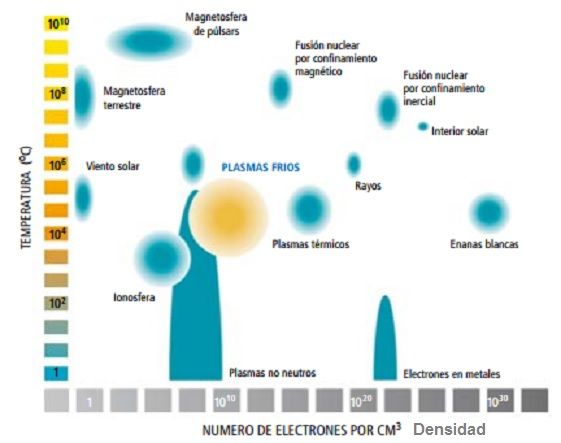
\includegraphics[height=7.8cm]{assets/figures/plasma.jpg}  
    \end{figure*}


%-------------Final de monografíaa--------------%
\section*{Conclusi\'on}

En conclusión, los campos de los materiales inteligentes, nanotecnología y plasma representan áreas de investigación y desarrollo de vanguardia que han transformado la manera en que interactuamos con la ciencia, la tecnología y la medicina. Estas disciplinas han demostrado ser fundamentales para abordar desafíos complejos y aprovechar oportunidades emocionantes en diversos sectores.

Los materiales inteligentes, con su capacidad para responder y adaptarse a estímulos externos, han abierto nuevas posibilidades en áreas como la electrónica, la medicina y la ingeniería. Desde polímeros con memoria de forma hasta sensores avanzados, estos materiales ofrecen soluciones innovadoras para problemas cotidianos y aplicaciones de vanguardia.

La nanotecnología, al operar a una escala nanométrica, ha permitido la manipulación precisa de la materia para crear materiales con propiedades extraordinarias. Desde dispositivos electrónicos más eficientes hasta avances en medicina personalizada, la nanotecnología ha demostrado su versatilidad y potencial para impactar positivamente en la sociedad.

Por otro lado, el plasma, ese estado de la materia altamente energético y conductor eléctrico, ha encontrado aplicaciones en campos tan diversos como la fusión nuclear, la tecnología de pantalla y la desinfección médica. Su capacidad para generar condiciones extremas y reacciones únicas lo convierte en una herramienta esencial en la investigación científica y la ingeniería de procesos avanzados.

En conjunto, estos campos están interconectados de manera fascinante. La nanotecnología ha permitido el desarrollo de materiales inteligentes a nivel nanométrico, mientras que el plasma se utiliza en procesos de fabricación y tratamiento que involucran nanomateriales. La convergencia de estos campos promete seguir impulsando la innovación, la eficiencia y la mejora de la calidad de vida en el futuro.

A medida que avanzamos en estas áreas de investigación, es fundamental abordar no solo los aspectos técnicos, sino también considerar las implicaciones éticas, sociales y medioambientales. El impacto de estos avances no solo radica en su capacidad para transformar industrias, sino también en su potencial para abordar desafíos globales de manera sostenible.
\bibliography{referencias}


\end{document}